% Compile: tectonic fig_ccmp_biology_ot_iclr.tex
% Editable TikZ; native drawing width = 5.5 in (ICLR text width).
% Query: 10.1021_acsomega.5c12723
% Gold: 10.1007/s11263-023-01831-9
% Data: drive_scan_sir4_biology/hops_{frame_ccmp,frame_ccmp_off,openie}.json
% Frame paths: top two simple seed-to-gold paths, with exact node labels.
% OpenIE: top-weighted simple path. A second path differs only in the
% direction of "equivalent" and is omitted for clarity.
% On/off uses the same trained weights. OpenIE is a separate model.
% Gates are CCMP-on sender gates, displayed to four decimal places.
% CCMP off applies g=1 even though its diagnostic logs retain predictions.
% Do not attribute the entire rank change to these paths alone.
\documentclass[border=2mm]{standalone}
\usepackage{xcolor,tikz,graphicx,caption,lmodern,helvet}
\usetikzlibrary{arrows.meta,calc}
\captionsetup{font=small,labelfont=bf,skip=6pt}
\definecolor{otInk}{HTML}{202A35}
\definecolor{otMuted}{HTML}{54616E}
\definecolor{otLine}{HTML}{C6CED5}
\definecolor{otOrange}{HTML}{955919}
\definecolor{otOrangeFill}{HTML}{FCF1E4}
\definecolor{otGreen}{HTML}{256D58}
\definecolor{otGreenFill}{HTML}{ECF5F0}
\definecolor{otPurple}{HTML}{675184}
\definecolor{otPurpleFill}{HTML}{F1EDF7}
\definecolor{otBlue}{HTML}{315F87}
\definecolor{otBlueFill}{HTML}{EEF4FA}
\definecolor{otGrayFill}{HTML}{F5F6F7}
\newcommand{\otFont}{\fontencoding{T1}\fontfamily{phv}\selectfont}
\newcommand{\otType}[2]{{\fontsize{6.8}{8}\selectfont\bfseries\color{#1}#2}}
\begin{document}
\begin{minipage}{139.7mm}
\centering
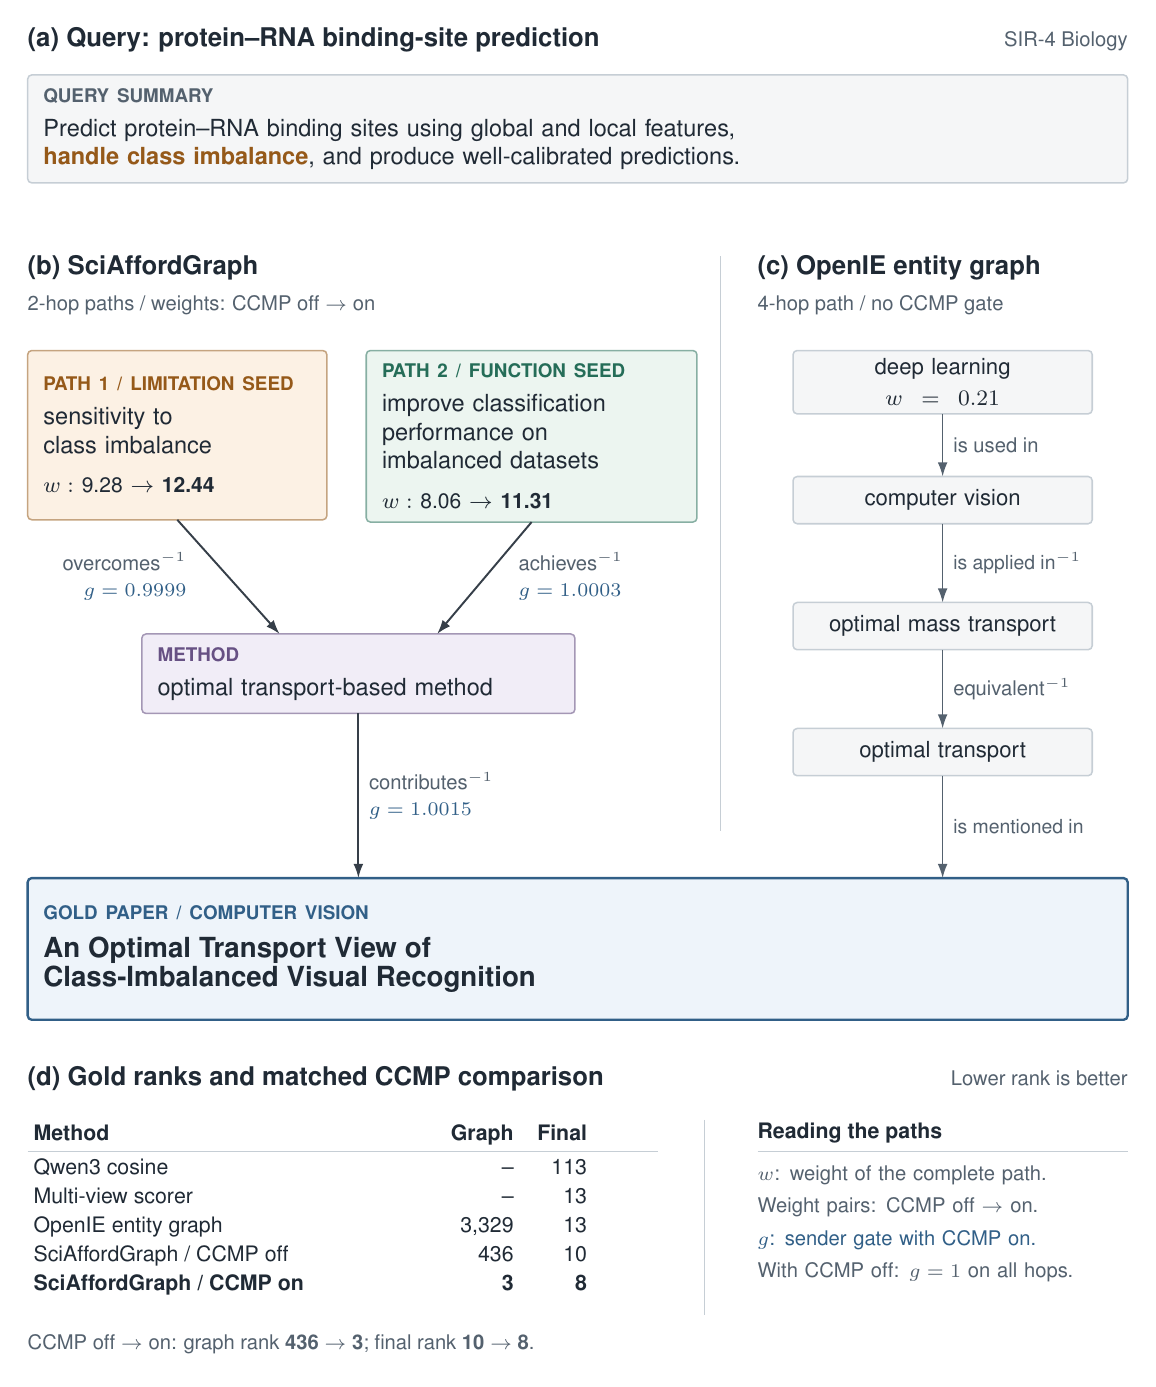
\begin{tikzpicture}[
 x=1mm,y=-1mm,font=\otFont\fontsize{8.5}{10.3}\selectfont,text=otInk,
 every node/.style={inner sep=0pt,outer sep=0pt,align=left,
   execute at begin node={\hyphenpenalty=10000\exhyphenpenalty=10000}},
 heading/.style={anchor=north west,font=\otFont\fontsize{9.3}{11}\selectfont\bfseries},
 note/.style={font=\otFont\fontsize{7.3}{8.7}\selectfont,text=otMuted},
 box/.style={draw=otLine,line width=.55pt,rounded corners=1.5pt,
   inner xsep=2mm,inner ysep=1.7mm,anchor=north,align=left},
 lim/.style={box,draw=otOrange!55,fill=otOrangeFill,text width=34mm},
 fun/.style={box,draw=otGreen!55,fill=otGreenFill,text width=38mm},
 method/.style={box,draw=otPurple!60,fill=otPurpleFill,text width=51mm},
 entity/.style={box,fill=otGrayFill,minimum height=6mm,
   inner xsep=1.5mm,inner ysep=1mm,text width=35mm,align=center,
   font=\otFont\fontsize{8}{9.5}\selectfont},
 edge/.style={-{Latex[length=1.8mm,width=1.25mm]},line width=.7pt,draw=otInk!90},
 oe/.style={edge,line width=.55pt,draw=otMuted},
 rel/.style={font=\otFont\fontsize{7.3}{8.5}\selectfont,text=otMuted,
   fill=white,inner sep=1pt},
]
\path[use as bounding box] (0,0) rectangle (139.7,169);

% Query text is an explicitly marked summary with its central need highlighted.
\node[heading] at (0,0) {(a) Query: protein--RNA binding-site prediction};
\node[note,anchor=north east] at (139.7,.5) {SIR-4 Biology};
\node[box,anchor=north west,fill=otGrayFill,text width=135.7mm] at (0,6)
 {\otType{otMuted}{QUERY SUMMARY}\\[2pt]
 Predict protein--RNA binding sites using global and local features,\\
 {\color{otOrange}\bfseries handle class imbalance}, and produce well-calibrated predictions.};

% Contrast specific typed relations against the recorded entity path.
\node[heading] at (0,29) {(b) SciAffordGraph};
\node[note,anchor=north west] at (0,34) {2-hop paths / weights: CCMP off $\rightarrow$ on};
\node[heading] at (92.7,29) {(c) OpenIE entity graph};
\node[note,anchor=north west] at (92.7,34) {4-hop path / no CCMP gate};
\draw[otLine,line width=.5pt] (88,29) -- (88,102);

\node[lim,minimum height=21.5mm] (s1) at (19,41)
 {\otType{otOrange}{PATH 1 / LIMITATION SEED}\\[2pt]
 sensitivity to\\class imbalance\\[4pt]
 {\fontsize{7.6}{9}\selectfont $w:$ 9.28 $\rightarrow$ \textbf{12.44}}};
\node[fun,minimum height=21.5mm] (s2) at (64,41)
 {\otType{otGreen}{PATH 2 / FUNCTION SEED}\\[2pt]
 improve classification\\performance on\\imbalanced datasets\\[4pt]
 {\fontsize{7.6}{9}\selectfont $w:$ 8.06 $\rightarrow$ \textbf{11.31}}};
\node[method] (m) at (42,77)
 {\otType{otPurple}{METHOD}\\[2pt]
 optimal transport-based method};
\draw[edge] (s1.south) -- (m.north -| 32,0);
\draw[edge] (s2.south) -- (m.north -| 52,0);
\node[rel,anchor=east,align=right] at (20.5,69.7)
 {overcomes$^{-1}$\\[1pt]{\color{otBlue}$g=0.9999$}};
\node[rel,anchor=west] at (62,69.7)
 {achieves$^{-1}$\\[1pt]{\color{otBlue}$g=1.0003$}};

\node[entity] (e0) at (116.2,41)
 {deep learning\\[2pt]{\fontsize{7.6}{9}\selectfont $w=0.21$}};
\node[entity] (e1) at (116.2,57) {computer vision};
\node[entity] (e2) at (116.2,73) {optimal mass transport};
\node[entity] (e3) at (116.2,89) {optimal transport};
\draw[oe] (e0.south) -- node[rel,right=1mm] {is used in} (e1.north);
\draw[oe] (e1.south) -- node[rel,right=1mm,font=\otFont\fontsize{7}{8.3}\selectfont] {is applied in$^{-1}$} (e2.north);
\draw[oe] (e2.south) -- node[rel,right=1mm] {equivalent$^{-1}$} (e3.north);

% The common gold is a cross-field destination, not another intermediary.
\node[box,anchor=north west,text width=135.7mm,fill=otBlueFill,draw=otBlue,
 line width=.85pt,minimum height=18mm] (gold) at (0,108)
 {\otType{otBlue}{GOLD PAPER / COMPUTER VISION}\\[2pt]
 {\fontsize{10}{11.8}\selectfont\bfseries An Optimal Transport View of\\Class-Imbalanced Visual Recognition}};
\draw[edge] (m.south) -- node[rel,right=1mm]
 {contributes$^{-1}$\\[1pt]{\color{otBlue}$g=1.0015$}} (gold.north -| 42,0);
\draw[oe] (e3.south) -- node[rel,right=1mm,font=\otFont\fontsize{7}{8.3}\selectfont] {is mentioned in} (gold.north -| 116.2,0);

% Rank and attribution tables use separate headers and aligned numeric columns.
\node[heading] at (0,132) {(d) Gold ranks and matched CCMP comparison};
\node[note,anchor=north east] at (139.7,132.5) {Lower rank is better};
\node[anchor=north west] at (0,138.7) {\otFont\fontsize{7.7}{9.5}\selectfont
\renewcommand{\arraystretch}{1.10}\setlength{\tabcolsep}{0pt}
\begin{tabular}{@{}p{53mm}r@{\hspace{3mm}}r@{}}
\textbf{Method} & \textbf{Graph} & \textbf{Final}\\[2pt]
Qwen3 cosine & -- & 113\\
Multi-view scorer & -- & 13\\
OpenIE entity graph & 3,329 & 13\\
SciAffordGraph / CCMP off & 436 & 10\\
\textbf{SciAffordGraph / CCMP on} & \textbf{3} & \textbf{8}\\
\end{tabular}};
\draw[otLine,line width=.55pt] (0,142.7) -- (80,142.7);
\draw[otLine,line width=.4pt] (86,138.7) -- (86,163.5);
\node[anchor=north west,font=\otFont\fontsize{7.7}{9.5}\selectfont\bfseries]
 at (92.7,139.1) {Reading the paths};
\draw[otLine,line width=.55pt] (92.7,142.7) -- (139.7,142.7);
\node[note,anchor=north west,text width=46mm] at (92.7,144.5)
 {$w$: weight of the complete path.\\[3pt]
 Weight pairs: CCMP off $\rightarrow$ on.\\[3pt]
 {\color{otBlue}$g$: sender gate with CCMP on.}\\[3pt]
 With CCMP off: $g=1$ on all hops.};
\node[note,anchor=north west] at (0,166) {CCMP off $\rightarrow$ on: graph rank \textbf{436 $\rightarrow$ 3}; final rank \textbf{10 $\rightarrow$ 8}.};
\end{tikzpicture}\par
\captionof{figure}{\textbf{Retrieving a vision method for a biological prediction problem.}
Two class-imbalance seeds converge on the method contributed by the gold paper.
The OpenIE path starts from the generic entity ``deep learning.'' CCMP on/off uses
identical trained weights; final denotes fused rank for graph methods.
Path weights $w$ are gradient attributions, with scales that differ across models.
Sender gates $g$ are shown to four decimal places for CCMP on; CCMP off applies $g=1$.
The displayed paths alone do not explain the full rank change. $r^{-1}$ denotes an inverse relation.}
\end{minipage}
\end{document}
